\section{Interestingness}
\label{sec:interestingness}

A major challenge when generating conjectures is choosing how to focus attention
on only those deemed ``interesting'' (either by avoiding uninteresting search
paths, and/or by filtering down the eventual output), since this is an imprecise
term with many different interpretations. For example, all existing approaches
agree that simple tautologies are ``uninteresting'', but differ when it comes to
more complex statements.  Colton~\etal{} surveyed tools for theory formation
and exploration, and their associated notions of ``interestingness'', for
concepts and conjectures~\cite{colton2000notion}. Six qualities were identified,
which are applied to conjectured properties as follows:

{\bf Empirical plausibility} checks whether a property holds across some
specific examples. This is especially useful for avoiding falsehoods, without
resorting to a deductive proof search.

{\bf Novelty} depends on whether the property, or one isomorphic or more
general, has already been seen.

{\bf Surprisingness} of a property is whether or not it is ``obvious'', for
example if it is an instance of a tautology.

{\bf Applicability} depends on the number of models in which a
property holds. High applicability makes a property more interesting, but so
does zero applicability (i.e. non-existence).

{\bf Comprehensibility} depends on the syntactic complexity of the property's
statement. Simpler statements are considered more interesting (which favours
tools adopting a small-to-large search order).

{\bf Utility} is the relevance or usefulness of a property to the user's
particular task. For example, if we want to find properties which are useful for
optimisation, like Equation~\ref{eq:mapreduce}, then utility would include
whether the property justifies some rewrite rule, the difference in resource
usage of the expressions involved, and how common those expressions are in real
usage.

\begin{table}
  \centering
  \scalebox{0.9}{
    \begin{tabular}{ |l|l|c|c|c|c|c|c| }
      \hline
      \multirow{2}{*}{\textbf{Program}}                      &
      \multirow{2}{*}{\textbf{Conjecture Types}}             &
      \multicolumn{6}{c|}{\textbf{Interestingness Measures}} \\ \hhline{~~------}
      \tRow{             &                     & \iE & \iN & \iS & \iA & \iC & \iU}
      \tRow{AM           & \tIFF, \tIMP, \tNE  &   X &   X &   X &   X &   X &   X}
      \tRow{GT           & \tIFF, \tIMP, \tNE  &   X &   X &   X &   X &   X &   X}
      \tRow{Graffiti     & \tINE               &   X &   X &   X &     &   X &   X}
      \tRow{\Bagai{}     & \tNE                &     &   X &     &   X &   X &    }
      \tRow{HR           & \tIFF, \tIMP, \tNE  &   X &   X &   X &   X &   X &   X}
      \tRow{\quickspec{} & \tEQ                &   X &   X &     &   X &   X &    }
      \tRow{\speculate{} & \tCON\ \tEQ / \tINE &   X &   X &     &   X &   X &    }
      \tRow{\isacosy{}   & \tEQ                &   X &   X &     &   X &   X &   X}
      \tRow{\isascheme{} & \tEQ                &   X &   X &     &   X &   X &   X}
    \end{tabular}
  }
  \caption{Classification of MTE tools from~\cite{colton2000notion}, extended
    to include four more recent tools. The interestingness measures are
    \iE{}mpirical plausibility, \iN{}ovelty, \iS{}urprisingness,
    \iA{}pplicability, \iC{}omprehensibility (low complexity) and \iU{}tility.}
  \label{table:colton}
\end{table}

% JUSTIFICATIONS
%
% ICoSy uses counter-example checking; this ensures empirical plausibility
% ICoSy uses constraints to avoid special-cases; this ensures novelty
% ICoSy uses utility, since there are some hard-coded patterns which are
% looked for
%
% Speculat uses a form of unification to ensure novelty, making sure one
% equation is not a special-case of another
% Speculat uses LeanCheck to enumerate values, looking for counterexamples
% Speculat uses testing, to ensure Empirical Plausibility
%
% QSpec uses QCheck to ensure empirical plausibility
% QSpec uses a congruence closure algorithm to ensure novelty
%
% IScheme uses utility, since it determines the "quality" of a definition
% based on how many theorems it appears in?
% IScheme uses novelty, using an equational rewrite system (Knuth-Bendix
% completion) to remove redundancies
% IScheme uses utility, since it focuses on the terms and definitions of a
% user's theory. However, don't all of them?
% IScheme uses counterexample checking for empirical plausibility.

% ONLY APPLIES TO PRECONDITIONS
% APPLICABILITY: ensure a conjecture holds in many models (or exactly zero, in
% the case of Bagai et al). Does the testing-based approach of QuickSpec and
% Speculate ensure that there's a model? After all, these are concrete values
% rather than e.g. implications of some abstract specification.

% FIXME: Give brief description and reference for each system in the text.
% We could include the more lengthy descriptions of IsaCoSy and QuickSpec here?

We summarise the criteria in Table~\ref{table:colton} and state which were used
in key ATF/MTE tools. The entries for AM, GT, Graffiti, \Bagai{} and HR are
based on this survey (the latter is Colton's own tool). The remaining rows are
our extension of this analysis to the (higher-order) tools we have focused on
(based on our understanding of their function): \quickspec{}~\cite{QuickSpec},
\speculate{}~\cite{braquehais2017speculate},
\isacosy{}~\cite{Johansson.Dixon.Bundy:conjecture-generation}
and \isascheme{}~\cite{Montano-Rivas.McCasland.Dixon.ea:2012}.

These recent tools all use testing to check for counterexamples, which ensures
results are empirically plausible and applicable (conditions are satisfiable,
types are inhabited, etc.). They also use a small-to-large search order,
ensuring more easily-comprehensibile conjectures are explored first.

\isacosy{} ensures novelty using a constraint system to prevent special-cases
being generated, whilst the others use post-hoc filters based on unification and
term rewriting to achieve the same result. \isacosy{} is able to look for
commonly desirable patterns, such as commutativity and associativity, which
increases the utility of its output, whilst \isascheme{} is completely based
around such pattern-instantiation.

This diversity of approaches makes it difficult to compare the existing
evaluations of these tools directly. In particular, evaluation methods created
for one tool might not make sense for another, due to assumptions made about
the algorithms' operation. For example, the novelty filters used by \quickspec{}
and \speculate{} are applied to the whole output set, guaranteeing that no
special-cases will appear; yet we cannot assume this in the case of \isacosy{},
since its constraint solver allows special cases if they're found \emph{before}
the general case (it does not go back and discard previous results).

In addition, attempting to \emph{measure} these qualities directly is difficult,
and having too many measures complicates comparisons. System developers have
employed a more practical alternative in their evaluations, which is to perform
\emph{precision/recall} analysis against a \emph{ground-truth}. This requires
choosing a set of definitions and a set of properties (the ground truth) which
represent the ``ideal'' result of conjecture generation for those definitions.
To analyse the quality of a tool's conjectures, we run it on these chosen
definitions and compare its output to the ground truth:

\begin{itemize}
\item \emph{Precision} is the proportion of a tool's output which appears in
  the ground truth (the ratio of true positives to all positives). This
  penalises overly-liberal tools which output a large number of properties in
  the hope that some turn out to be ``good''.
\item \emph{Recall} is the proportion of the ground truth which appears in the
  tool's output (the ratio of true positives to actual positives). This
  penalises overly-conservative tools which generate very few properties as a
  way to avoid ``bad'' ones.
\end{itemize}

To score 100\% on precision and recall, all of the properties which appear in
the ground truth must have been conjectured, and nothing else. This gives us a
simple method to evaluate and compare tools without requiring a general solution
to the question of what is ``interesting''; although we must still decide what
to put in the ground truth set, and what to leave out, for each measured set of
definitions.

The precision/recall analysis shown in~\cite{claessen2013automating} is the only
quantitative comparison of recent MTE tools we have found in the literature.
Our Theory Exploration Benchmark, described in section~\ref{sec:benchmark}, is
essentially an extension of this approach, to a larger and more diverse set of
examples.

\subsection{Exploration in Theorem Proving}
\label{sec:examples}

Conjecture generation (automated or manual) is crucial when formally proving
statements, such verifying software against its specification. This provides a
concrete, empirical setting to determine what makes statements interesting (at
least from a utilitarian point of view).

\paragraph{Generalisation}

\providecommand{\coq}[1]{\lstinline[language=ML]|#1|}

When we \emph{generalise} a statement $S$, we obtain a new statement $S'$ of
which $S$ is a special case. Although it seems counterintuitive, a generalised
statement can sometimes be \emph{easier} to prove than the original. This arises
often in inductive proofs (e.g. when reasoning about tail-recursive
definitions~\cite{kapur2003automatic}\footnote{Tail-recursive functions are
  desirable due to their constant space usage, unlike recursion in non-tail
  positions which requires a growing number of stack frames or nested closures.
  The presence of accumulator arguments makes reasoning harder, so it is common
  to use the direct implementation for proofs, then transport them over to the
  tail-recursive definition via an equivalence relation.}), since the specific
obligations which arise in the proof may be incompatible with the available
inductive hypotheses. An informative example is given by Boyer and Moore of the
associativity of multiplication in \textsc{ACL2}~\cite{boyer1983proof}:

$$(x * y) * z = x * (y * z)$$

During the course of the proof, the following obligation arises:

\begin{equation}
  \tag{conc3}
  (y + (x * y)) * z = (y * z) + ((x * y) * z)
  \label{eq:conc3}
\end{equation}

ACL2 automatically generalises \eqref{eq:conc3} by replacing the repeated
sub-term $x * y$ with a fresh variable $w$:

\begin{equation}
  \tag{conc4}
  (y + w) * z = (y * z) + (w * z)
  \label{eq:conc4}
\end{equation}

This generalised form is clearly the distributivity law for multiplication and
addition, which can be proved separately to the original goal of
associativity. It would not be controversial to claim that this distributivity
law is interesting in its own right (relative to associativity, at least), in
addition to its usefulness in making this proof go through.

% TODO: Describe the ACL2 heuristics

Generality hence contributes to a conjecture's \emph{utility}, and also (by
definition) to its \emph{applicability}. It is still important to balance
against other concerns, since blindly generalising \emph{all} statements or
proof obligations we come across would result in conjectures so strong that they
are unprovable, or even false; which would make them much less interesting.

\paragraph{Analogy}

The interestingness of a statement can also be characterised by \emph{analogy}
to existing interesting statements. By finding lemmas analogous to those of a
different theory, we may be able to re-use proof tactics and other forms of
meta-programming across both. In this case an analogy would map from a solved
problem to a currently-unproven goal, and applying this map to the lemmas
appearing in the existing proof allows us to infer the approximate form of the
lemmas required for the new theorem.

The approach taken by \textsc{ACL2(ml)} is to find lemmas which may be relevant
to solving a goal $G$ by making analogies via unsupervised
clustering~\cite{Heras.Komendantskaya.Johansson.ea:2013}. These clusters are
used in two ways:

\begin{itemize}
\item First, we use the cluster $C_G$ containing $G$ to identify analogous
  theorems.

\item For each theorem $T \in C_G \setminus \{G\}$, we consider those symbols
  $S_T$ which occur in $T$ but not in $G$. Our analogous lemmas are those used
  to prove $T$, mutated such that symbols $s \in S_T$ are replaced by members of
  the cluster $C_s$ containing $s$.
\end{itemize}

The interestingness of such generated lemmas derives from both the existence of
the original lemma (which is presumably interesting enough to prove and
subsequently explore), that of the target theorem it may help to prove, and the
novelty provided by reframing existing concepts in a new domain. The running
examples for demonstrating \textsc{ACL2(ml)} are equivalence theorems for
tail-recursive definitions with their direct (non-tail-recursive) counterparts,
as well as the effect of repeating certain list operations:

\begin{itemize}
\item
  $\forall n, \texttt{natp}(n) \rightarrow \texttt{fact-tail}(n) =
  \texttt{fact}(n)$ where \texttt{natp} is the predicate that $n$ is a natural
  number, whilst \texttt{fact-tail} and \texttt{fact} are tail-recursive and
  non-tail-recursive implementations of factorial, respectively.

\item
  $\forall n, \texttt{natp}(n) \rightarrow \texttt{power-tail}(n) =
  \texttt{power}(n)$, where \texttt{power-tail} and \texttt{power} calculate
  powers of 2.

\item
  $\forall n, \texttt{natp}(n) \rightarrow \texttt{fib-tail}(n) =
  \texttt{fib}(n)$, where \texttt{fib-tail} and \texttt{fib} calculate fibonacci
  numbers.

\item
  $\forall x, \texttt{nat-listp}(x) \rightarrow \texttt{sort}(\texttt{sort}(x))
  = \texttt{sort}(x)$, for list-of-natural-numbers predicate \texttt{nat-listp}
  and list-sorting function \texttt{sort}.

\item
  $\forall x, \texttt{true-listp}(x) \rightarrow \texttt{rev}(\texttt{rev}(x)) =
  x$, where \texttt{true-listp} ensures that $x$ is a valid singly-linked list
  structure and \texttt{rev} is list reversal.

\item $\forall x, \texttt{true-listp}(x) \rightarrow \texttt{int}(x, x) = x$,
  where \texttt{int} is the intersection of lists (i.e. a list of elements
  common to each).
\end{itemize}

\paragraph{Auxiliary Lemmas} \label{sec:auxiliarylemmas}

One consideration when generating conjectures is the difference between
theorems, lemmas, corollaries, etc. From a logical point of view, these are all
equivalent, and hence most proof assistants do not distinguish between
them. However, their \emph{intention} may be different: in a sense, theorems are
the interesting results; whilst lemmas are useful results, required for proving
the theorems. Corollaries are consequences and special-cases of theorems, which
are interesting enough to state separately, but not as much as a theorem.

Some systems, like Coq, allow users to \emph{label} each statement as being a
\coq{Theorem}, a \coq{Lemma}, etc. despite their internal representations being
the same. This shows us immediately that lemmas outnumber theorems; in the Coq
standard library there are over five times as many lemmas as theorems
\footnote{Coq version \texttt{8.4pl6} contains (excluding comments) 1492
  occurences of \coq{Theorem} and 7594 of \coq{Lemma} in its \texttt{theories/}
  directory.}.

% TODO: Analyse them

% TODO: Theory exploration as lemma generation; give example from a HipSpec paper

We can find a need for auxiliary lemmas, once again, in the context of
tail-recursive functions. Consider proving the (pointwise) equality of the
following Coq functions, defined for the Peano naturals \coq{Z} and \coq{S}:

\begin{coqblock}
Inductive Nat : Set := Z : Nat
                     | S : Nat -> Nat.

Fixpoint plus      (n m : Nat) := match n with
                                      | Z    => m
                                      | S n' => S (plus n' m)
                                  end.

Fixpoint plus_tail (n m : Nat) := match n with
                                      | Z    => m
                                      | S n' => plus_tail n' (S m)
                                  end.
\end{coqblock}

These definitions are equivalent to the following Haskell:

\begin{haskell}
plus :: Nat -> Nat -> Nat
plus      Z      m = m
plus      (S n') m = S (plus n' m)

plus_tail :: Nat -> Nat -> Nat
plus_tail Z      m = m
plus_tail (S n') m = plus_tail n' (S m)
\end{haskell}

Both of these functions implement addition, but the \coq{plus_tail} variant is
tail-recursive. However, if we want to \emph{prove} that the definitions are
(pointwise) equal, we run into difficulties. In particular, when the inductive
step requires us to prove \coq{plus (S n) m = plus n (S m)} (which seems
reasonable), we cannot make this go through using another inductive argument.

\begin{coqblock}
(* Solve equalities by beta-normalising both sides *)
Ltac triv := try (simpl; reflexivity).

(* Prove equivalence of plus and plus_tail *)
Theorem equiv : forall n m, plus n m = plus_tail n m.
  induction n; triv. (* Base case is trivial *)

  (* Inductive case: plus (S n) m = plus_tail (S n) m *)
  intro m.

  (* Beta-reduce the right-hand-side (justification is trivial) *)
  replace (plus_tail (S n) m) with (plus_tail n (S m)); triv.

  (* Use induction hypothesis to replace plus_tail with plus *)
  rewrite <- (IHn (S m)).
\end{coqblock}

Specifically, the \emph{conclusion} of a second inductive hypothesis is exactly
the equation we need:

\begin{coqblock}
IHn' : (forall x, plus n' x = plus_tail n' x) -> plus (S n') m = plus n' (S m)
\end{coqblock}

Yet we cannot provide it with the argument it needs, as our original induction
hypothesis is \emph{too specific} (it has too many \coq{S} constructors):

\begin{coqblock}
IHn : forall x, plus (S n') x = plus_tail (S n') x
\end{coqblock}

We are forced to abandon the proof, despite such a reasonable-looking
intermediate goal.

In fact, if we attempt to prove that goal \emph{separately}, we can use a
straightforward argument by induction; even though it is actually
\emph{stronger} due to the absence of the \coq{IHn} assumption:

\begin{coqblock}
Lemma gen n m : plus (S n) m = plus n (S m).
  induction n; triv. (* Base case is trivial *)

  (* Move all S constructors outside *)
  simpl. rewrite <- IHn. simpl.

  (* Trivial *)
  reflexivity.
Defined.
\end{coqblock}

Using this separate result as a lemma, the orignal pointwise equality is proven
easily:

\begin{coqblock}
  rewrite (gen n m).
  reflexivity.
Defined.
\end{coqblock}

Hence demonstrating the utility, and therefore interestingness, of such
auxilliary lemmas.

% TODO Include Colton/Bundy et al

\subsection{Tests}

Since we are working in the domain of Haskell programs, an abundant source of
statements are available in the form of \emph{tests}. For manually-written
tests, the effort required to write them implies that they must be of some
interest to their author. Many forms of test are \emph{not} suitable for our
purposes, such as \emph{unit tests} which are always trivially provable by
$\beta$-reduction; or \emph{integration tests}, which depend on the behaviour of
the external environment. One reason to study Haskell is its widespread use of
\emph{property checking}, which does give us useful data in the form of
universally quantified statements. Many Haskell property checkers exist, based
on random testing (\quickcheck{}~\cite{claessen2011quickcheck} and
\smartcheck{}~\cite{pike2014smartcheck}), enumeration
(\smallcheck{}~\cite{runciman2008smallcheck}), observation
(\lazysmallcheck{}~\cite{reich2013advances}) and logic programming
(\sparsecheck{}~\cite{sparsecheck}).

Thankfully the major differences between these systems are in the way they
instantiate test arguments; their representations of properties are largely the
same (modulo renaming of functions and types): as Haskell functions with free
variables encoded as function arguments.

\subsection{Artificial Curiosity} \label{sec:intrinsic}

\begin{figure}
  \centering
  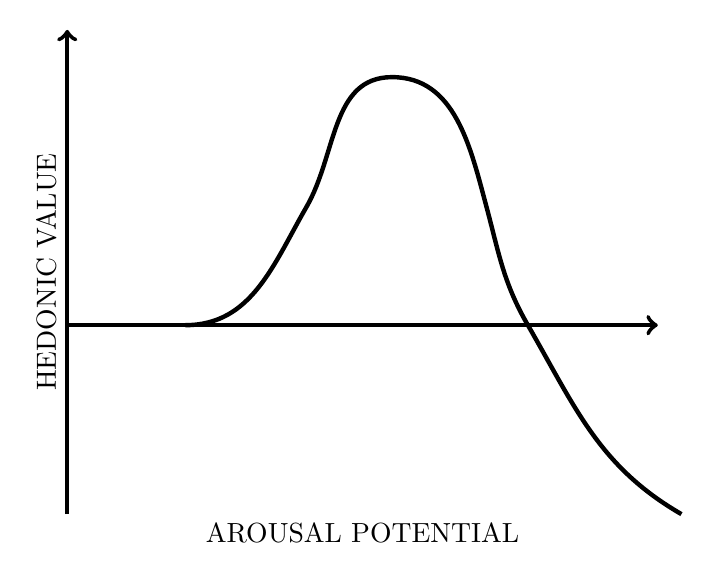
\begin{tikzpicture}[scale=0.75]
      % The image, for reference
      % \node[anchor=south west,inner sep=0] at (0,0) {\includegraphics[width=\textwidth]{wundt.png}};

      % Axes
      \draw[black,ultra thick,->] (1,0.8) -- (1,  9)   node[midway, above, sloped] {HEDONIC VALUE};     % y axis
      \draw[black,ultra thick,->] (1,4)   -- (11, 4);                                                   % x axis
      \path                       (1,0.8) -- (11, 0.8) node[midway, below]         {AROUSAL POTENTIAL}; % x axis label

      % Curve. The numbers come from tracing over wundt.png
      \draw[black,ultra thick] (3, 4)
           to[out=0,   in=240] (5.05, 6)
           to[out=60,  in=180] (6.5,  8.2)
           to[out=0,   in=105] (8.1,  6)
           to[out=-75, in=120] (8.8,  4)
           to[out=-60, in=150] (11.4, 0.8);

      % This version is closer, but a little jagged
      \iffalse
      \draw[black,ultra thick] (3, 4)
           to[out=0,   in=240] (5.05, 6)
           to[out=60,  in=225] (6,    8)
           to[out=45,  in=180] (6.5,  8.2)
           to[out=0,   in=135] (7.2,  8)
           to[out=-45, in=105] (8.1,  6)
           to[out=-75, in=120] (8.8,  4)
           to[out=-60, in=150] (11.4, 0.8);
      \fi
  \end{tikzpicture}

  \caption{The Wundt curve, reproduced from~\cite{berlyne1970novelty}. The axes
    ``hedonic value'' and ``arousal potential'' are described as covering
    \textquote{reward value\dots preference or pleasure}, and \textquote{all the
      stimulus properties that tend to raise arousal, including novelty and
      complexity}, respectively.}
  \label{fig:wundt}
\end{figure}

Another perspective on what is ``interesting'' comes from the artificial
intelligence tasks of optimisation and reinforcement learning. Common pitfalls
for such systems are highly non-convex problems (trapping optimisers in local
minima), and sparse information (such as flat gradients; or highly delayed
rewards, like a single win/lose reward at the end of a game). To mitigate these problems, various forms of internally-generated (or \emph{intrinsic}) rewards
can be incorporated into a system. Such schemes provide reward for interesting
discoveries, which encourages exploration in lieu of external direction, and are
known as \emph{Artificial Curiosity}~\cite{schmidhuber2006developmental} (AC).

The unifying principle of AC methods is to force systems away from data which
are not amenable to learning; either because they are so familiar that there is
nothing left to learn, or so unfamiliar that they are unintelligible. The
resulting behaviour is characterised by the \emph{Wundt curve} (shown in Figure \ref{fig:wundt}) \footnote{In practice, many measures
  avoid negative values for simplicity, in which cases we replace all negative
  points on the curve with zero.}, which has been used in psychology to explain
human aesthetics and preferences \cite{berlyne1970novelty}. This same behaviour
may be applicable to the theorems produced by a theory exploration system.

We can divide AC approaches into two groups: those which make \emph{explicit}
use of interestingness, learning from signals which follow a Wundt curve; whilst
\emph{implicit} approaches modify the \emph{output} of their learning
algorithm(s), to engineer the overall system behaviour to follow a Wundt curve
as an emergent property.

A framework encompassing many examples of the explicit approach is given
in~\cite{oudeyer2007intrinsic} in the context of reinforcement learning; for
comparison, many similar measures are surveyed in a data mining context
in~\cite{geng2006interestingness}. Many more reinforcement learning examples can
be found in~\cite{Kaplan2006, Lipson2007, Luciw2011, Macedo2000,
  Ramik.Sabourin.Madani:2013, Roa.Kruijff.Jacobsson:2009, Schmidhuber:1991,
  oudeyer2004intelligent}; whilst more general descriptions are given
in~\cite{Schaul.Sun.Wierstra.ea:2011, Scott1989, maher2008achieving}, which may
be more amenable to Theory Exploration setting.

Many of these reward signals are based on information theory, with a prominent
example being \emph{compression progress}: given a compressed representation of
our previous observations, the ``progress'' is the space saved if we include the
current observation. Observations which are incompressible or trivially
compressible don't save any space, whilst observations which provide new
insights into the structure of past experience can provide a space saving when
compressed together. This seems particularly relevant for identifying
interesting theorems: those new theorems (``observations'') which shorten the
proofs of previously discovered theorems may be more general, more powerful and
therefore more \emph{interesting}. In fact this is very similar to
\quickspec{}'s interestingness criterion.

Another example of explicit Artificial Curiosity is given
in~\cite{Hester.Stone:2012}, where world states which cause \emph{disagreement}
among a population of decision trees (a \emph{random
  forest}~\cite{randomforests}) are considered interesting. Since the models
make stochastic predictions, the disagreement follows a Wundt curve as the
complexity of state transitions increases: for parts of the state space which
have been fully learned, the models will agree on accurate predictions; for
parts which are unlearnable, the models cannot infer any structure, and will
converge to reporting the same average value. Whilst the latter predictions may
not be \emph{accurate}, they will be \emph{in agreement}, hence pushing down the
interestingness of states which are too complex.

Many examples of the implicit case are based on \emph{coevolution}: rewarding
one part of the system for exploiting another part, and vice versa. In~\cite{Schmidhuber1999} a pair of learning algorithms place virtual ``bets''
on the outcome of actions, and the winner is rewarded at the expense of the
loser. Due to the risk involved, each algorithm will only bet when it is
confident in its prediction, and bets will only be actioned when each algorithm
is confident in a \emph{different} outcome. The overall behaviour of this system
is therefore similar to the explicit measure of disagreement used in the random
forest example.

More recent work on \emph{Generative Adversarial Networks} (GANs) trains a
``discriminator'' program to distinguish real training examples (usually images)
from synthetic data made by a ``generator'' program. Both programs are
differentiable (usually some type of Artificial Neural Network), so the coupling
between the generator's output and the discriminator's input can be used not
only to feed synthetic data ``forwards'', but also to back-propagate the
discriminator's errors (which it is trying to minimise) into the generator
(which then tries to maximise, exploiting the discriminator by synthesising more
realistic data).

Another example of implicit AC is the ``darwinian brain'' of Fernando et
al.~\cite{fernando2013design1, fernando2013design2}. This coevolves a
population of problem generators and problem solvers, rewarding the solvers
based on their speed, and rewarding the generators based on the \emph{variance}
of the solvers' speed. This avoids trivial problems (which all solvers can
quickly overcome) and complex problems (which no solver can manage), and focuses
on those with the most possibility for learning. The role of problem generator
is similar to that of Theory Exploration tools, with solvers being Automated
Theorem Provers.

% TODO Include something about
% variance among experts (decision tree stuff as well as more established
% splitting functions stuff)

% TODO: Also mention the intrinsic reward idea about easily accessible regions
% (e.g. balancing a pole because it's easier to get from there to anywhere else)

% TODO Make sure we mention the recent reinforcement learning task that includes
% a constantly-changing "TV" in the 3D world, shown in some TwoMinutePapers
% videos
